\documentclass{sig-alternate}
\usepackage{graphicx}
\usepackage{amsmath}
\usepackage{amssymb}


\title{Model-Based Auto-Tuning}

\numberofauthors{3}

\author{
%\alignauthor First Last\titlenote{}\\
\alignauthor First Last\\
\affaddr{Affiliation line 1}\\
\affaddr{Affiliation line 2}\\
\email{anon@mail.com}
% 2nd author
%\alignauthor First Last\titlenote{None}\\
\alignauthor First Last\\
\affaddr{Affiliation line 1}\\
\affaddr{Affiliation line 2}\\
\email{anon@mail.com}
% 3rd author
%\alignauthor First Last\titlenote{None}\\
\alignauthor First Last\\
\affaddr{Affiliation line 1}\\
\affaddr{Affiliation line 2}\\
\email{anon@mail.com}
}

\begin{document}
\maketitle

\begin{abstract}
Each generation of GPU hardware presents unique programming challenges.
It is difficult to write software that obtains good performance on a range of hardware.

Auto-tuning is an effective technique for adapting a parametrized
GPU code template to current hardware.

Autotuning, however, is a relatively expensive kernel-selection mechanism - it
works by actually running the desired GPU computation in tens or hundreds of
ways before selecting the best implementation strategy for a particular
machine.

Futhermore library abstraction boundaries provide operations such as image
filtering and matrix multiplication, which actually correspond to a large set
of possible computations: for example the correlation of 1 large image with 1
small filters is  quite a different computational problem than the correlation
of 100 small images with 10 large filters.
This paper considers (XXX) strategies for using previous auto-tuning
measurements from similar problems to short-circuit computationally
expensive auto-tuning on a new problem of interest.

This paper presents a machine learning approach to generalized auto-tuning, in
which features of
(a) the current hardware platform,
(b) the kernel configuration
and (c) the problem instance are used to fit a regression model that predicts
how fast an implementation is (XXX).
We argue that autotuning using this surrogate model can be effective, while
being much faster than normal auto-tuning.

Whereas auto-tuning on problem XXX takes XXX seconds, our approach obtains
(XXX) of the speed in (XXX) of the time.


XXX: Hill-climbing (HC) search is effective alternative to grid.
XXX: How is HC search affected by mutation rate?
XXX: Purely random search is not an effective alternative to grid.

\end{abstract}


\section{Introduction}

There is a natural function from
problem space x implementation space x platform space to runtime:
how much wall time elapses on the given platform when solving the given
problem with the given implementation.

Autotuning is a family of empirical techniques for finding the implementation
that minimizes that runtime function, when the platform and the problem
configuration are given.

XXX: some math, or possibly a picture with the three boxes that was on Pinto's
whiteboard.

This paper is about different ways of doing the minimization.
For a particular problem (filterbank correlation) we
look at a parameterized kernel implementation (from GCG)
and a few hardware platforms, and compare
random search, grid search, and a hill-climbing strategy with a good, but
generic, reference implementation.
Then we show that we can model the LSM function with a regression tree
well enough to usefully perform the argmin of Equation~\ref{eq:lsm_argmin}
on the model rather than the actual system. Whereas it may take several
minutes to perform a hill-climbing or grid search in the original system,
a hill-climbing search in the model requires a small fraction of a second.
Model-based autotuning makes it possible to simulate auto-tuning quickly and
accurately enough to be used within a single library call of the computational
routine.



\subsection{Problem Space: Filter-bank Correlation}

Our experiments on automatic auto-tuning will be focused on filterbank
correlation.  Mathematically, we define filterbank correlation in terms of an
image $x$ and a filterbank $f$.
The image $x$ has $R$ rows, $C$ columns, and $D$ channels (e.g. color
channels) that we call its {\em depth}. We index $x$ like $\mathbf{x}[i,j,d]$
where $1 \leq i \leq R$ and $1 \leq j \leq C$.
The filterbank $f$ has $K$ square filters of side-length $W$, each one of
which has $D$ channels.
The result of filterbank correlation of $x$ with $f$ is an image-like array
$z$ with $R-W+1$ rows, $C-W+1$ columns, and depth $K$, whose elements are
defined according to Equation~\ref{eq:z}:

\begin{equation}
    \mathbf{z}[i,j,k] = \sum_{u=1}^{W} \sum_{v=1}^{W} \sum_{d=1}^D
        \mathbf{x}[i+u, j+v, d]~ \mathbf{f}[k, u, v, d].
        \label{eq:z}
\end{equation}

Filterbank correlation is used extensively in image and video processing,
where it is often the computational bottleneck.
GPUs are well-suited to computing filterbank correlations, although the
optimal strategy for doing so often depends on the shape of the problem, i.e.
the choices of $R$, $C$, $D$, $F$, and $W$.

We randomly sampled problem specifications from the following space:
\begin{figure}
\begin{center}
\begin{minipage}{.4\textwidth}
\begin{verbatim}
R : one_of(256, 512, 1024, 2048, 4096)
D : one_of(1, 4, 8, 16, 32, 64, 128, 256)
F : one_of(1, 4, 8, 16, 32, 64, 128, 256)
W : one_of(3, 5, 7, 9, 11)
\end{verbatim}
\end{minipage}
\end{center}
\caption{The full configuration space for filterbank correlation included a
total of 1600 elements, but we restricted our experiments to problems that
represented between 1 and 50 gigaflops. Our problem space included 602
configurations. In a full application in which all image and filter sizes are
valid, the number of configurations would be effectively infinite.
XXX: define R, D, F, W here
}
\label{fig:probspace}
\end{figure}
% Problems were considered invalid if the filters were larger than the images.
% but in the new setting with iheight >= 256 this never happened.
Problems were tested if they represented between 1 and 50 gigaflops.  Problems
that were smaller do not fully utilize the hardware, and are handled equally
well by many kernel settings, including the reference (XXX cite GCG).
Problems that were larger take so long to evaluate that there is negligible
inefficiency in implementing them via multiple calls with smaller images and fewer filters.
The configuration space described in Figure~\ref{fig:probspace} included 602
configurations with between 1 and 50 gigaflops.

In a full, reusable, library implementation of the filter correlation
operation, we would also provide options for arbitrary image shapes,
arbitrary integer depth and filter shapes, and also support a variety of
physical input layouts via strides.  These additional options would make our
approach of automatic auto-tuning even more important, because there would be
a greater variety in the kinds of computations and memory transfers to
perform.  In our experiments, we only consider the problem variations
described in Figure ~\ref{tbl:}, which already suffice to show that automatic
auto-tuning is a promising approach.


\subsection{Kernel Space: Metaprogramming}

\begin{figure}
\begin{center}
\begin{minipage}{.43\textwidth}
\begin{verbatim}
block_w   : one_of(4, 8, 16, 32, 64, 128)
block_h   : one_of(4, 8, 16, 32, 64, 128)
n_filter_r: one_of(1, 2)
n_output4s: one_of("all", 1, 2)
spill     : one_of(False, True)
imul_fast : one_of(False, True)
pad_shared: one_of(False, True)
use_tex1d : one_of(False, True)
maxrreg   : one_of(8, 16, 20, 24, 28, 32, inf)
fast_math : one_of(False, True)
\end{verbatim}
\end{minipage}
\end{center}
\caption{The kernel used to perform
filterbank correlation was parametrized by 10 parameters, some of which
were binary and others of which were integer-valued. The full configuration
space included 12000 kernels.
XXX: how to make sense of these paramters without code listing?
}
\end{figure}

XXX: What to all the parameters mean?
XXX: Point to github / GCG for full code listing.

XXX: how many configurations are in the configuration space

XXX: what was the reference kernel, and how was it chosen?

\iffalse
\subsection{Platform Space: XXX}

XXX: GCG chapter pg 13 notes that among the grid search, the best parameter
setting is different for the various platforms.

XXX: so far we only tried 3 cards... so we're using a 1-of-N feature.
\fi


\section{Results}

\subsection{Random, Grid, and Hill-Climbing Search}

XXX: Histogram (over problems) of gigaflops/sec of random, grid, random,
hill-climbing for each/selected platform.
This shows that our implementations and problems are stressing the cards,
that our implementation is pretty good, and that different problem sizes pose
different computational challenges.

XXX: Scatterplot of gigaflops vs. gigaflops / second (of best grid point)
should show that it's not just problem size that makes it possible to go fast.


XXX: histogram of speedups of grid, random, hill-climbing over reference, for
several hardware platforms. (GET ANOTHER -- macbook??)
Sometimes the reference implementation is optimal, in many cases it is far
from optimal: Which cases? What's wrong with the reference?

TL;DR: Hill-climbing is a good way to search the implementation space, can
search the full space and do about as well as grid search in the more
restricted space.

\begin{figure}
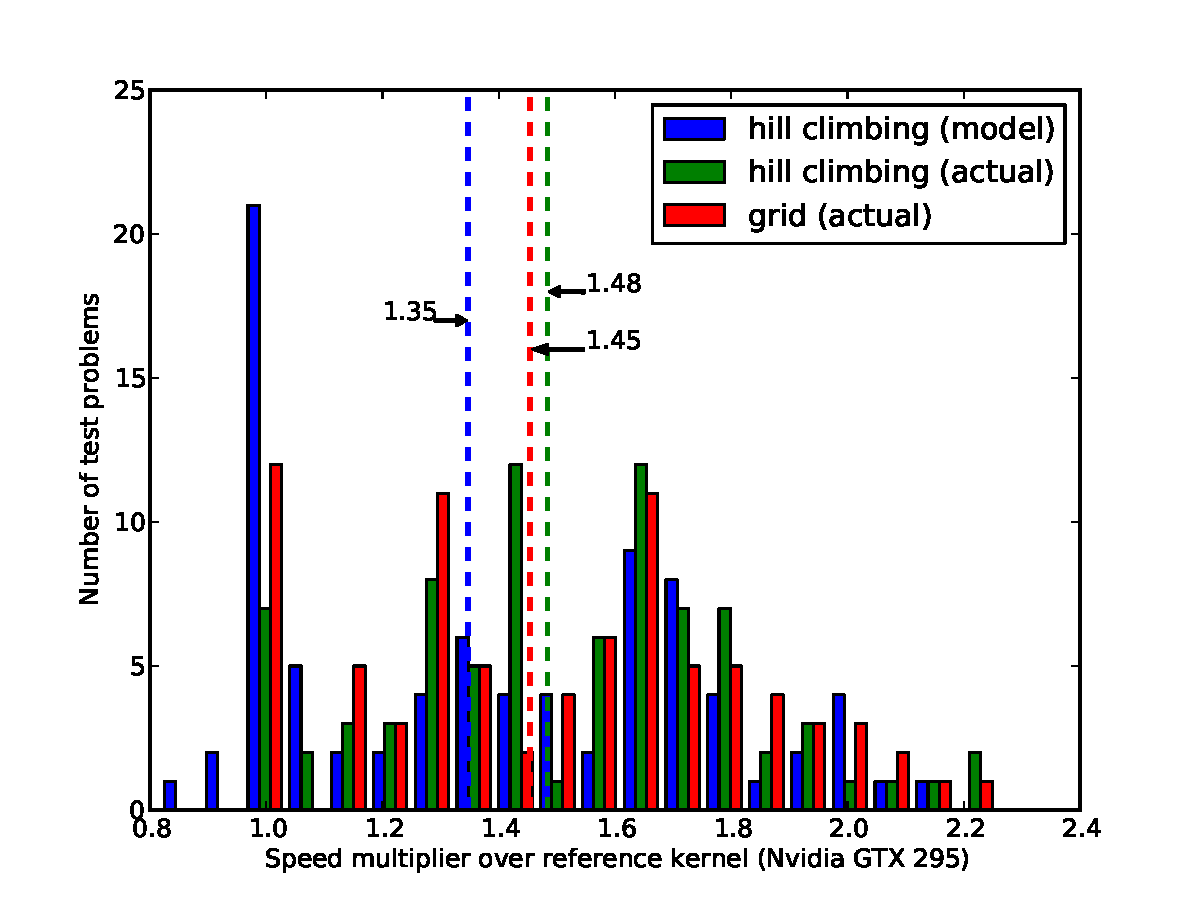
\includegraphics[scale=.5]{speedup_295.pdf}
\caption{Speedup of various auto-tuning strategies over a good reference
implementation.
Each strategy was evaluated the same set of 83 problem configurations, which
was disjoint from the problem configurations used to build the model for
model-based hill-climbing.
The vertical dashed lines are positioned at the geometric mean speedup (XXX?)
of each strategy. The grid and hill-climbing approaches
tested 73 and 75 configurations respectively, and took 45?? XXX
seconds on average.
The model-based approach tested 0 configuration evaluations, and took 0.05
seconds on average, even with a naive Python implementation.
}
\label{fig:speedup_295}
\end{figure}


\subsection{Model-based Autotuning}

On the GTX 295, a single decision-tree fit to the log-speed-multiplier
(LSM) function (XXX: how many problem configurations, how much vs. what
kind of training data) achieves an average Spearman correlation of 0.9 on
held-out test data (XXX: what kind of test data).

Now: the big test is that if we use the genetic search on the model instead of
the original function, do we get good performance?

\section{Discussion}

We're characterizing hardware by a 1-of-N feature vector, simply describing
which hardware is the current hardware.
To make better use of auto-tuning data from other platforms, it would be more
useful to have precise and descriptive features such as: what compute
capability is present, how many cores are active, what is the bandwidth
between the various kinds of memory, and how much of various kinds of memory
is present.  With these features a model-assisted auto-tuning approach
might be able to make very good guesses on hardware for which no auto-tuning
has ever been done.

\end{document}
